\section{Overview}

In hybrid virtual environments, RDMA virtualization not only needs to maintain high performance and manageability, but also have generality for hybrid virtual environments. Therefore, our RDMA virtualization goals are as follows:

\begin{itemize}
\item {\verb|Generality|}: To form unified RDMA virtualization, single centralized virtual layer should be set up, which is provided to virtual machines and containers with general interfaces.
\item {\verb|High performance|}: Virtual RDMA should be close to native RDMA in terms of throughput, latency, and CPU load. Meanwhile it should be suit for large-scale virtual cluster.
\item {\verb|High manageability|}: In RDMA virtualization, container and virtual machine characteristics should be maintained to realize portability, isolation and network management.
\end{itemize}

To achive unified RDMA virtualization for hybrid virtual environment,  we propose a software RDMA virtualization framework, namely uniRDMA. The vRNIC constructed by uniRDMA based on the user space virtualization layer provides unified virtual RDMA.

As Figure~\ref{fig:framework-overview} shows, uniRDMA is consist of two parts: uniRDMA user space virtual layer and uniVerbs interface. The former is responsible for the establishment and management of virtual RDMA. The specific work includes the virtualization of vRNIC, the mapping management of vRNIC to VF, and the virtual RDMA network management, such as virtual RDMA address configuration and routing; the latter is mainly aout how RDMA applications use vRNICs, including the construction of general interfaces and the optimization.

\begin{figure}[!ht]
	\centering
	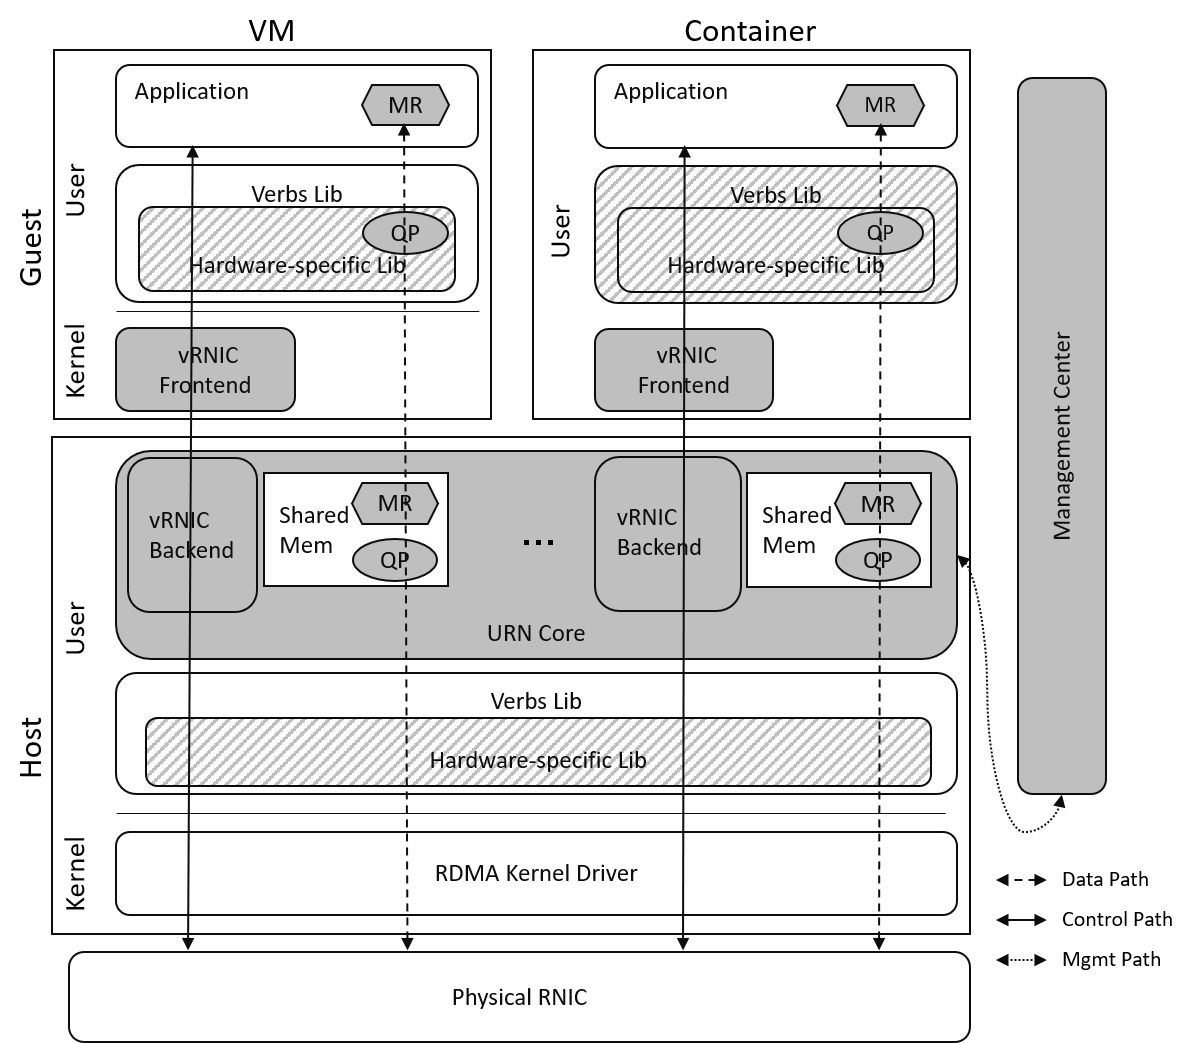
\includegraphics[width=0.9\linewidth]{images/framework-overview}
	\caption{uniRDMA Framwork Overview}
	\label{fig:framework-overview}
\end{figure}
